% !TEX TS-program = pdflatex
% !TEX encoding = UTF-8 Unicode


%\documentclass[12pt,a4paper]{memoir} % for a long document
%\documentclass[12pt,a4paper,article]{memoir} % for a short document
\documentclass[12pt,a4paper]{article}

\usepackage[utf8]{inputenc} % set input encoding to utf8


%%% PACKAGES
\usepackage{booktabs} % for much better looking tables
\usepackage{graphicx} % support the \includegraphics command and options
\usepackage{array} % for better arrays (eg matrices) in maths
\usepackage{paralist} % very flexible & customisable lists (eg. enumerate/itemize, etc.)
\usepackage{verbatim} % adds environment for commenting out blocks of text & for better verbatim
\usepackage{listings} % for code segment environments.
% see http://en.wikibooks.org/wiki/LaTeX/Source_Code_Listings
\usepackage{tikz} % for FSM drawings from http://madebyevan.com/fsm/
\usepackage{qtree} % for \Tree
\usepackage{float} % unlocks [H] for float-placement.
\usepackage{subcaption} % unlocks the subfigure environment
\usepackage{multirow} % allows columns and rows to span multiple rows and colums, respectively
\usepackage{fancyhdr} % unlocks pagestyle 'fancy' and \[lcr](foot|head)
\pagestyle{fancy} 
\usepackage{fullpage}

%\setcounter{secnumdepth}{3}

\renewcommand\thesubsubsection{\alph{subsubsection})} % changes the subsubsection numbering to %LETTER%)

\usepackage[parfill]{parskip} % Activate to begin paragraphs with an empty line rather than an indent

\setlength{\headheight}{15pt} % distance between top of page and header
\setlength{\headsep}{30pt} %distance between the page text and header
\pagestyle{fancy} 
%\renewcommand{\headrulewidth}{0pt}

\title{TDT4205 Compiler Design\\
\textbf{Problem set 5, Theory, Assembly}}
\author{Odd M. Trondrud}
%\date{} % Delete this line to display the current date

\lhead{TDT4205 Compiler Design, Spring 2014}
\chead{}
\rhead{\texttt{trondrud}}




%%% BEGIN DOCUMENT
\begin{document}

\newpage
\maketitle
%\tableofcontents* % the asterisk means that the contents itself isn't put into the ToC


% problem 1
\section{Optimization}
Explain each of the following optimizations and show how they can be used to improve the three-address flow graph.
Start with the original flow graph for each case.

\emph{Note: I use ``Bn.m'' to refer to line m in block n of the original flow graph.}
\subsection{Common subexpression elimination}
% CU lecture 23
% DB pg 588
From \textsc{the Dragon Book}, page 588:
\begin{quote}
``An occurrence of an expression \emph{E} is called a common subexpression if \emph{E} was previously computed and the values of the variables in \emph{E} have not changed since the previous computation.''
\end{quote}

You'd think \textit{B3.6} contains a common subexpression, since \texttt{i + t} is also computed at \textit{B3.2}.
However \textit{B3.2} changes the value of \texttt{i}, so while the expression in \textit{B3.6} was previously computed, the values of the variables have changed and therefore it is not a common subexpression.

\subsection{Copy propagation}
% CU lecture 23
% DB pg 590
``After an assignment, \texttt{x = y}, replace references to \texttt{x} with \texttt{y} until \texttt{x} is assigned something else.''
In this quote, taken from the 23rd CU lecture slides, \texttt{y} probably denotes a variable rather than an expression as replacing a variable with an expression would muck up the three-address code format.

This optimization would change \textit{B3.5} to \texttt{d = i + 2}.

You'd think we should also change \textit{B3.2} to \texttt{i = 1 + t}, because of the assignment in \textit{B1.1}, but doing so would gunk up the code because control can enter \textit{B3} through more than one path ($\mathit{B1} \rightarrow \mathit{B2} \rightarrow \mathit{B3}$ and $\mathit{B3} \rightarrow \mathit{B2} \rightarrow \mathit{B3}$).

\subsection{Code motion}
% DB pg 592
This is when we move the evaluation of a statement that doesn't change over time out of the body of the loop so that it's only computed once rather than once per iteration of the loop.

This optimization would move \textit{B3.1} and \textit{B3.4} to \textit{B1}.

\subsection{Dead code elimination}
% DB pg 591

Dead code elimination is when we remove statements whose effects are never observed in the code.
E.g. if we've got two different assignments to the same variable without the variable ever being referenced in-between the two assignments, then we can remove the first assignment as its effect is never observed.

This would remove \textit{B3.4}. 

% problem 2
\newpage
\section{[More] Optimization}
Consider the following C-code:
\begin{lstlisting}[language=C, tabsize=4, basicstyle=\ttfamily\small]
for (int i =0; i < n; i++) {
	sum = 4 * i;
	for (int j = 0; j < m; j = j + i) {
		a = a + b * 2;
	}
}
\end{lstlisting}

\subsection{In the context of optimization, what is an induction variable, and what is reduction in strength?}
% DB pg 592
\paragraph{Induction variable}
A variable $x$ is said to be an ``induction variable'' if there is a constant $c \in \mathbb{R}$ such that each time $x$ is assigned, its value increases by $c$.

\texttt{i}, as in the textbook example and programmer's favourite loop-counter-variable, is an induction variable.
Who knows how that came to be?
Is it because of those Fortran-people being math-people and mathematicians use $i$ in their sums and matrix indexes?
Does it stand for ``\textbf{i}ndex''?
Oh convention, you are surely the mother of some confusion.

\paragraph{Reduction in strength}
In the context of optimization, it is the replacement of ``expensive'' operations (such as multiplication and division) by a cheaper one (such as addition or subtraction).

\subsection{Convert the code above to a three-address flow graph.}
% I could use flow (http://ctan.mackichan.com/support/flow/flowdoc.pdf) for this
% or I could man up and do it with TikZ, but then I'd have to learn TikZ.
%	http://www.texample.net/tikz/examples/simple-flow-chart/
% Ooorr apparently I could use graphviz. I already sort-of know graphviz, so hmm.
% man, so many choices.
% fuck it let's just use TikZ
%	http://www.texample.net/media/pgf/builds/pgfmanualCVS2012-11-04.pdf
\begin{figure}[H]
\centering
	% hurp a derp a tikz flow graph

\tikzstyle{block} = [rectangle, draw, font=\ttfamily\small]
\tikzstyle{arrow} = [draw, -latex']
\tikzstyle{label} = [font=\fontshape{it}\selectfont] % labels are in italics

\begin{tikzpicture}[node distance = 2cm, auto]
	% code blocks
	\node[block] (B1) 				{i = 0};
	\node[block, below of=B1] (B2) 	{if i < n goto B3};
	%	edge[arrow, bend right=45] (B1.east);
	\node[block, below of=B2] (B3)	{\makecell[l]{c = 4 * i\\j = 0}};
	\node[block, below of=B3] (B4)	{\makecell[l]{if j < m goto B5}};
	\node[block, below of=B4] (B5)	{\makecell[l]{d = b * 2 \\a = a + d \\j = j + i}};
	\node[block, below of=B5] (B6)	{i = i + 1};
	\node[block, below of=B6] (B7)	{ };
	% labels
	\node[label, left of=B1] 		{B1};
	\node[label, left of=B2] 		{B2};
	\node[label, left of=B3]		{B3};
	\node[label, left of=B4]		{B4};
	\node[label, left of=B5]		{B5};
	\node[label, left of=B6]		{B6};
	\node[label, left of=B7]		{B7};
	% edges
	\path	(B1)		edge	[arrow, bend right=0]	node	{}	(B2);
	\path	(B2)		edge	[arrow]					node	{}	(B3);
	\path	(B3)		edge	[arrow]					node	{}	(B4);
	\path	(B4)		edge	[arrow]					node	{}	(B5);
	\path	(B6.east)	edge	[arrow, bend right=45]	node	{}	(B2);
	\path	(B2.east)	edge	[arrow, bend left=55]	node	{}	(B7.east);
	\path	(B4.east)	edge	[arrow, bend left=30]	node	{}	(B6);
	\path	(B5.west)	edge	[arrow, bend left=50]	node	{}	(B4.west);
\end{tikzpicture}

\caption{A three-address flow graph for the code in Problem 2.}
\label{fig:2-b}
\end{figure}

\subsection{Optimize the flow graph by performing strength reduction on induction variables, and removing unnecessary induction variables.}
% strength reduction on the induction variables
% remove unnecessary induction variables

% sum = 4*i ==> sum = sum + 4
% j is only used for the comparison in block 3
% i is used in the computation of j and in the comparison in block 2
Ok so for the $n$th iteration of the inner loop, the value of \texttt{j} is $j_n$ where $j_n = j_{n-1} + i$ and $j_1 = 0$.
If we work upwards from $j_1$, we see that $j_n = (n-1)*i$.
I'm not sure if it helps, though.
All I managed to do with that was replace \texttt{j = i + j} with \texttt{j = i * n} where \texttt{n} is a new induction variable that increases by 1 for each iteration of the inner loop.
But not only does that introduce a new induction variable, it's also the opposite of strength reduction.
So I didn't do that.

I did do code movement and pulled \texttt{d = b * 2} out of the loop body and also reduced it to \texttt{d = b << 1}.

Also I replaced the multiplication in the assignment of \texttt{sum} with addition.
% d = b << 1
% i also did code motion

\begin{figure}[H]
\centering
	% hurp a derp a tikz flow graph

\tikzstyle{block} = [rectangle, draw, font=\ttfamily\small]
\tikzstyle{arrow} = [draw, -latex']
\tikzstyle{label} = [font=\fontshape{it}\selectfont] % labels are in italics

\begin{tikzpicture}[node distance = 2cm, auto]
	% code blocks
	\node[block] (B1) 				{\makecell[l]{i = 0 \\c = - 4 \\d = b << 1}};
	\node[block, below of=B1] (B2) 	{if i < n goto B3};
	%	edge[arrow, bend right=45] (B1.east);
	\node[block, below of=B2] (B3)	{\makecell[l]{c = c + 4 \\j = 0}};
	\node[block, below of=B3] (B4)	{\makecell[l]{if j < m goto B5}};
	\node[block, below of=B4] (B5)	{\makecell[l]{a = a + d \\j = j + i}};
	\node[block, below of=B5] (B6)	{i = i + 1};
	\node[block, below of=B6] (B7)	{ };
	% labels
	\node[label, left of=B1] 		{B1};
	\node[label, left of=B2] 		{B2};
	\node[label, left of=B3]		{B3};
	\node[label, left of=B4]		{B4};
	\node[label, left of=B5]		{B5};
	\node[label, left of=B6]		{B6};
	\node[label, left of=B7]		{B7};
	% edges
	\path	(B1)		edge	[arrow, bend right=0]	node	{}	(B2);
	\path	(B2)		edge	[arrow]					node	{}	(B3);
	\path	(B3)		edge	[arrow]					node	{}	(B4);
	\path	(B4)		edge	[arrow]					node	{}	(B5);
	\path	(B6.east)	edge	[arrow, bend right=45]	node	{}	(B2);
	\path	(B2.east)	edge	[arrow, bend left=55]	node	{}	(B7.east);
	\path	(B4.east)	edge	[arrow, bend left=30]	node	{}	(B6);
	\path	(B5.west)	edge	[arrow, bend left=50]	node	{}	(B4.west);
\end{tikzpicture}

\caption{An optimized version of the three-address flow graph in Figure~\ref{fig:2-b}.}
\label{fig:2-c}
\end{figure}

% problem 3
\newpage
\section{Data-flow analysis}
\subsection{In the context of reaching definition analysis, what does it mean for a definition to reach a point in the code?}
% I guess it's time to read 9.2 of DB
% pg 598: a variable may be defined by one of [some number of points in the code]. The definitions that may reach a program point along some path are known as reaching definitions.
% So if we're at some point X in the code, then all the definitions at points that might be included in the path to X are reaching definitions? ok I think I got that
% ooh so if the set of reaching definitions for variable x only has one member at a point Y then we can replace x by that definition at point Y (constant folding!)
If a definition for some variable $x$ reaches a point $p$ in the code, then there exists a path from the definition to $p$ on which there are no other definitions of $x$.
The definitions need not be constants ($x$ could be assigned another variable, for instance).
However if there is only one reaching definition for $x$ at a point right before $x$ is referenced then it's possible to replace $x$ with that definition.
If the definition is a constant it's called \emph{constant folding}.
If it's a variable it is called \emph{copy propagation}.

\subsection{Perform reaching definitions data-flow analysis by computing the \emph{gen, kill}, IN and OUT sets for each block of the flow graph above.}
% IN[s] = data-flow values before statement s
% OUT[s] = data-flow values after statement s
% data-flow value = abstract representation of the set of all possible program states that can be observed for a given point/statement

% transfer function of definition d: u = v + w (i.e. d is a definition of u)
% f_d(x) = gen_d \union (x - kill_d)
%	gen_d = {d}, kill_d = all other definitions of u in the program
% the fuck is x, though? Is it a point?

%anyway, gen(Block) is the set of all definitions that reach the end of the block, yeah?
% Definitions of gen and kill for basic blocks on pg 605 of DB
% kill(Block) is the union of all the definitions killed by the individual statements
% gen(Block) contains all the definitions inside the block that are "visible" immediately after the block -- we refer to them as 'downwards exposed'.
%	a definition is downward exposed if it is not overwritten by another definition below it

% so I just need to figure out what IN[Block] and OUT[Block] is
%pg 606:
% OUT[B] = gen(B) U (IN[B] - kill(B))
% IN[B]  = U_P OUT[P]
% the last one means that IN[B] is equal to the union of the OUT sets of blocks P that are direct predecessors of B
% "A - B" is the set of elements that are in A but not in B
% A U \emptyset = A

% I just learned how to do this!
\newcommand{\IN}[1]{\text{IN[#1]}}
\newcommand{\OUT}[1]{\text{OUT[#1]}}

So $gen(\text{B})$ is the set of all definitions inside block B that reach the end of the block and $kill(\text{B})$ is the union of all the definitions killed by the individual statements in the block.
Note that according to Figure 9.13 on page 604 it would seem that the domain of $kill(\text{B}$ is all definitions in the program (or CFG, whichever).

IN[B] and OUT[B] are defined as
$$\OUT{B} = gen(B) \cup (\IN{B} - kill(B))$$
$$\IN{B} = \bigcup_{P}\OUT{P}$$
Where P is a predecessor block of B and I'm guessing the big cup thing is supposed to be like a sum except instead of addition it performs union?
It's from page 605 of \textsc{BOOK OF DRAGONS}.

Also
$$\OUT{ENTRY} = \emptyset$$

In addition I'd guess $gen(\text{EXIT})$ and $kill(\text{EXIT})$ are undefined or whatever because with this definition of OUT,
computing \OUT{EXIT} doesn't make much sense since it's dependent on both $gen(\text{EXIT})$ and $kill(\text{EXIT})$ and the EXIT block itself is empty so...
oh, wait, I guess that means that $\OUT{EXIT} = \emptyset \cup (\IN{EXIT} - \emptyset) = \IN{EXIT}$.

An algorithm for computing the IN and OUT sets for the blocks of a CFG can be found in Figure 9.14 on page 607 of \textsc{You know which book}.
That's the one I used to figure out the values seen in Table~\ref{tab:3-b-1}~through~\ref{tab:3-b-3}.
Well actually I stopped once I saw that \OUT{B1} was unchanged between Step 2 and 3, because the algorithm does say we should stop when there are no more changes to any OUT and since the OUT set of a block depends on its IN set which depends on the OUT set of its immediate predecessors I figured we wouldn't be seeing any more changes due to how the graph looks.
Yeah that's a rather convoluted explanation but I'm sure you know how it's supposed to work.

% man I am pretty lazy
\renewcommand\thesubsubsection{Step \arabic{subsubsection}}
\setcounter{subsubsection}{-1} % counters are apparently inserted as ++counter
% so if you want the first occurrence of it to be n, you have to set it to n-1
\subsubsection{\emph{gen} and \emph{kill} sets}

$gen(\text{B1}) = \{d_1,~d_2,~d_3\}$

$kill(\text{B1}) = \{d_5, ~d_6, ~d_8, ~d_{10}, ~d_{11}, ~d_{12}\}$

$gen(\text{B2}) = \{d_4,~d_5\}$

$kill(\text{B2}) = \{d_1,~ d_{10}\}$

$gen(\text{B3}) = \{d_6,~ d_7\}$

$kill(\text{B3}) = \{d_2,~ d_8\}$

$gen(\text{B4}) = \{d_8,~ d_9\}$

$kill(\text{B4}) = \{d_2,~ d_6\}$

$gen(\text{B5}) = \{d_{10},~ d_{12}\}$

$kill(\text{B5}) = \{d_1,~ d_3,~ d_5,~ d_{10},~ d_{11},~ d_{12}\}$

\subsubsection{First iteration}
% whoo-hoo! this is like using variables or whatever and generating the text!
% thug lyfe mofo
\newcommand{\INBone}	{$\emptyset$}
\newcommand{\OUTBone}	{$\{d_{1},~ d_2,~ d_3\}$}
\newcommand{\INBtwo}	{\OUTBone}
\newcommand{\OUTBtwo}	{$\{d_2,~ d_3,~ d_4,~ d_5\}$}
\newcommand{\INBthree}	{\OUTBtwo}
\newcommand{\OUTBthree}	{$\{d_3,~ d_4,~ d_5,~ d_6,~ d_7\}$}
\newcommand{\INBfour}	{\OUTBtwo}
\newcommand{\OUTBfour}	{$\{d_3,~ d_4,~ d_5,~ d_8,~ d_9\}$}
\newcommand{\INBfive}	{$\{d_3,~ d_4,~ d_5,~ d_6,~ d_7,~ d_8,~ d_9\}$}
\newcommand{\OUTBfive}	{$\{d_1,~ d_4,~ d_6,~ d_7,~ d_8,~ d_9,~ d_{10},~ d_{12}\}$}

\begin{table}[H]
\centering
\begin{tabular}{lcc}
	\toprule
	\textsc{Block}	& \textsc{IN}	& \textsc{OUT} \\
	\midrule
	B1	& \INBone	& \OUTBone	\\
	B2	& \INBtwo	& \OUTBtwo	\\
	B3	& \INBthree	& \OUTBthree\\
	B4	& \INBfour	& \OUTBfour	\\
	B5	& \INBfive	& \OUTBfive	\\
\end{tabular}
\label{tab:3-b-1}
\caption{Status of the IN and OUT sets at the end of step \arabic{subsubsection}.}
\end{table}


\subsubsection{Second iteration}
% can't use the values from the last step because LaTeX sees the re-definition of the commands
% before it sees their usage and apparently does lazy evaluation so the command inside the command isn't executed before the command is used, not when it is defined
% which, when you think about it, shouldn't be too surprising
% I guess I just wanted the compiler to know what I was thinking IS THAT TOO MUCH TO ASK
% HUH
\renewcommand{\INBone}		{$\{d_1,~ d_4,~ d_6,~ d_7,~ d_8,~ d_9,~ d_{10},~ d_{12}\}$}
\renewcommand{\OUTBone}		{$\{d_1,~ d_2,~ d_3,~ d_4,~ d_7,~ d_9\}$}
\renewcommand{\INBtwo}		{\OUTBone}
\renewcommand{\OUTBtwo}		{$\{d_2,~ d_3,~ d_4,~ d_5,~ d_7,~ d_9\}$}
\renewcommand{\INBthree}	{\OUTBtwo}
\renewcommand{\OUTBthree}	{$\{d_3,~ d_4,~ d_5,~ d_6,~ d_7,~ d_9\}$}
\renewcommand{\INBfour}		{\OUTBtwo}
\renewcommand{\OUTBfour}	{$\{d_3,~ d_4,~ d_5,~ d_7,~ d_8,~ d_9\}$}
\renewcommand{\INBfive}		{$\{d_3,~ d_4,~ d_5,~ d_6,~ d_7,~ d_8,~ d_9\}$}
\renewcommand{\OUTBfive}	{$\{d_4,~ d_6,~ d_7,~ d_8,~ d_9,~ d_{10},~ d_{12}\}$}

\begin{table}[H]
\centering
\begin{tabular}{lcc}
	\toprule
	\textsc{Block}	& \textsc{IN}	& \textsc{OUT} \\
	\midrule
	B1	& \INBone	& \OUTBone	\\
	B2	& \INBtwo	& \OUTBtwo	\\
	B3	& \INBthree	& \OUTBthree\\
	B4	& \INBfour	& \OUTBfour	\\
	B5	& \INBfive	& \OUTBfive	\\
\end{tabular}
\label{tab:3-b-1}
\caption{Status of the IN and OUT sets at the end of step \arabic{subsubsection}.}
\end{table}


\subsubsection{Third iteration}
\renewcommand{\INBone}		{$\{d_4,~ d_6,~ d_7,~ d_8,~ d_9,~ d_{10},~ d_{12}\}$}
\renewcommand{\OUTBone}		{$\{d_1,~ d_2,~ d_3,~ d_4,~ d_7,~ d_9\}$}

\begin{table}[H]
\centering
\begin{tabular}{lcc}
	\toprule
	\textsc{Block}	& \textsc{IN}	& \textsc{OUT} \\
	\midrule
	B1	& \INBone	& \OUTBone	\\
	B2	& \INBtwo	& \OUTBtwo	\\
	B3	& \INBthree	& \OUTBthree\\
	B4	& \INBfour	& \OUTBfour	\\
	B5	& \INBfive	& \OUTBfive	\\
\end{tabular}
\label{tab:3-b-1}
\caption{Status of the IN and OUT sets at the end of step \arabic{subsubsection}.}
\end{table}



\subsection{Explain how a compiler can use the results to determine that the variable \texttt{b} must be a constant at the start of the exit node.}
Oh, I forgot to compute \IN{EXIT} and \OUT{EXIT}.
Well $\IN{EXIT} = \OUT{B5}$.

\IN{EXIT} is computed the same way as any other IN set which, in our case, means it's equal to \OUT{B5}.
Looking at \OUT{B5} in Table~\ref{tab:3-b-3} reveals that it contains two definitions for the variable \texttt{b}: $d_6$ and $d_8$.
That means \texttt{b} could have either of these definitions as we reach the EXIT node.
But hey, \emph{wait a minute}, both $d_6$ and $d_8$ define \texttt{b} as a constant!
So that's how we know that the variable \texttt{b} must be a constant at the start of the exit node.
We don't know exactly \emph{which} constant it'll be, but it's either 5 or 4 which, y'know, is a smaller set than $\mathbb{Z}_{0}^{2^{32}-1}$ (or whatever, I don't know the type of \texttt{b}).


% problem 4
\section{Register allocation}
Consider the three address code:
\begin{lstlisting}[language=C, tabsize=2, basicstyle=\ttfamily\small, numbers=left, numberstyle=\small\color{gray}]
	a = b + c
	d = a + b
	e = 2 * a
	a = e + c
	b = d + a
	c = e - 2
\end{lstlisting}

\subsection{In the context of live variable analysis, what does it mean for a variable to be \emph{live} at a point in the code?}
% 9.2.5 Live-Variable Analysis, starts on pg 608
% In live variable analysis, we wish to know for a variable x and point p whether the value of x at p could be used along some path in the flow graph starting at p.
% if so, we say that x is live at p, otherwise, x is dead at p.
If a variable $x$ is live at a point $p$, then its value could be used (i.e. read before being assigned anew) along some path in the flow graph starting at $p$.

\subsection{Perform live variable analysis on the code above.}
% uh
% def_B = the set of variables defined (assigned values) in block B prior to any use of that variable in B
% use_B = the set of variables whose values may be used in B prior to any definition of the variable
% uh, the book says that any variable in use_B must be considered live on entrance to block B 
%  while any variable in def_B are definately dead at the beginning of B.
% which would mean that variables can be both dead and live at the beginning of B? what?
% oh no according to the definition of IN[B], membership in use_B has precedence over def_B

% IN[B] = set of variables live on entry from block B
% OUT[B]= set of variables live on exit from block B
Am I supposed to treat the entire code segment as a basic block?
Or should I treat each as a basic block?
Or should I make up some scheme to divide the lines into basic blocks?

If I just assume the entire segment is one basic block B then $\IN{B} = \{a,~b,~c,~d,~e\}$ and $\OUT{B} = \emptyset$.
And that doesn't really tell us much.
So let's do it line-by-line instead, ait?
Cool.
Well not \emph{cool}, it's going to take a bunch of time since I'm doing it by hand and I have to tabulate the results as well.
But cool, as in OK.

I'm treating each line as a basic block where block $n$ contains line $n$.
E.g. block 1 contains the statement \texttt{a = b + c}.


And for this answer I'd like to extend thanks to Algorithm 9.14 on page 610.
You know which book it's in.

\setcounter{subsubsection}{-1} % counters are apparently inserted as ++counter
\subsubsection{\emph{def} and \emph{use}}
\begin{table}[H]
\centering
\begin{tabular}{lcc}
	\toprule
	\textsc{Block}	& $use_b$	& $def_b$	\\
	\midrule
%	point	  use		  def 
	ENTRY	& 			&			\\
	1		& b, c		& a 		\\
	2		& a, b		& d			\\
	3		& a			& e			\\
	4		& c, e		& a			\\
	5		& a, d		& b			\\
	6		& e			& c			\\
	\bottomrule
\end{tabular}
\caption{\emph{def} and \emph{use} for the code segment in Problem 4.}
\label{tab:4-b-0}
\end{table}

% oh man can I just reuse the table template I made for problem 3?
% I think I can!
% Whooo!
% Well almost, I need to copy it and add a line due to a mismatch in the number of blocks
\subsubsection{Iteration one}
\newcommand{\INBe}			{b, c}
\newcommand{\OUTBe}			{b, c}
\renewcommand{\INBone}		{b, c}
\renewcommand{\OUTBone}		{a, b}
\renewcommand{\INBtwo}		{a, b}
\renewcommand{\OUTBtwo}		{a, d}
\renewcommand{\INBthree}	{a, d}
\renewcommand{\OUTBthree}	{a, d}
\renewcommand{\INBfour}		{a, d}
\renewcommand{\OUTBfour}	{a, d, e}
\renewcommand{\INBfive}		{a, d, e}
\renewcommand{\OUTBfive}	{e}
\newcommand{\INBsix}		{e}
\newcommand{\OUTBsix}		{$\emptyset$}
\begin{table}[H]
\centering
\begin{tabular}{lcc}
	\toprule
	\textsc{Block}	& \textsc{OUT}	& \textsc{IN} \\
	\midrule
	ENTRY	& \OUTBe	& \INBe		\\
	1		& \OUTBone	& \INBone	\\
	2		& \OUTBtwo	& \INBtwo	\\
	3		& \OUTBthree& \INBthree	\\
	4		& \OUTBfour	& \INBfour	\\
	5		& \OUTBfive	& \INBfive	\\
	6		& \OUTBsix	& \INBsix	\\
	\bottomrule
\end{tabular}
\caption{Status of the IN and OUT sets at the end of step \arabic{subsubsection}.}
\label{tab:\arabic{section}-\alph{subsection}-\arabic{subsubsection}} % man, LaTeX is /pretty cool/
% this should allow me to reference the tables by the number of subsubsection they're in. Which is cool.
\end{table}


Since there's only one possible path for control to flow in the code segment for this problem and it goes straight from ENTRY to EXIT, one iteration of Algorithm 9.14 is enough.


\subsection{Draw the register interference graph for the code above.}
% http://www.cs.cornell.edu/Courses/CS412/2008sp/lectures/lec33.pdf
% make a graph containing one node for each variable in the code
% For each IN and OUT set S from 4-b
% draw an edge between the variables in S

% time to bust out TikZ
\begin{figure}[H]
\centering
\tikzstyle{derp} = [circle, draw, font=\ttfamily\small]

\begin{tikzpicture}[every node/.style={draw, circle, minimum size=0.75cm}]
	\node				(a)		{a};
	\node[right of=a]	(b)		{b};
	\node[right of=b]	(c)		{c};
	\node[below of=a]	(d)		{d};
	\node[right of=d]	(e)		{e};

	\path
	(a) 	edge 	(b)
			edge	(d)
			edge	(e)
	(b)		edge 	(c)
	(d)		edge	(e);
\end{tikzpicture}

\caption{The register interference graph for the code above.}
\label{fig:4-c}
\end{figure}

\subsection{How many registers are needed to avoid register spills for the above code (assuming a hardware architecture capable of three-address code (e.g. ARM))?}
The minimum number of registers required to avoid register spilling is smallest possible number of different colors needed to color the register interference graph.
Since the graph is small we can attempt to 3-color\footnote{the number 3 was chosen randomly by fair dice roll} the graph and if we do we see that yes, there exists a solution.
Check out Figure~\ref{fig:4-d} for the answer.

\begin{figure}[H]
\centering
\tikzstyle{derp} = [circle, draw, font=\ttfamily\small]

\begin{tikzpicture}[every node/.style={draw, circle, minimum size=0.75cm}]
	\node							(a)		{a};
	\node[right of=a, fill=green]	(b)		{b};
	\node[right of=b]				(c)		{c};
	\node[below of=a, fill=green]	(d)		{d};
	\node[right of=d, fill=red]		(e)		{e};

	\path
	(a) 	edge 	(b)
			edge	(d)
			edge	(e)
	(b)		edge 	(c)
	(d)		edge	(e);
\end{tikzpicture}

\caption{3-coloring of the register interference graph.}
\label{fig:4-d}
\end{figure}

So: We need three registers in order to avoid register spills.
Any number higher than three will also let us avoid register spills, but three is the smallest possible number of registers required.


\end{document}
